In this task we will be investigating, analysing and crack the calculator,
getting its flag.

\section{Exploiting expensive\_calculator\_x86}
\label{s:exploiting}

Below there is a list of the tools used to perform the task.

\begin{description}[align=left]
  \item [Tools Used]
  \item [IDA Pro Hex Ray:] disassembler
  \item [GDB version:] GNU Debugger
  \item [Python:] to write the exploit, key generator and more
  \item [PwnTools:] a python library for solving pwnable challenges from CTFs
  \item [GEF:] to prettify GDB's text user interface.
  \item [ltrace:] to inspect library calls in a Linux executable
  \item [carbon:] to prettify the code through images and bring consistency to
  the report
\end{description}

\section{Investigation}
\label{s:investigation}

Let's start with identifying what type of file is this
expensive\_calculator\_x86 using the following command:
\begin{figure}[H]
  \centering
  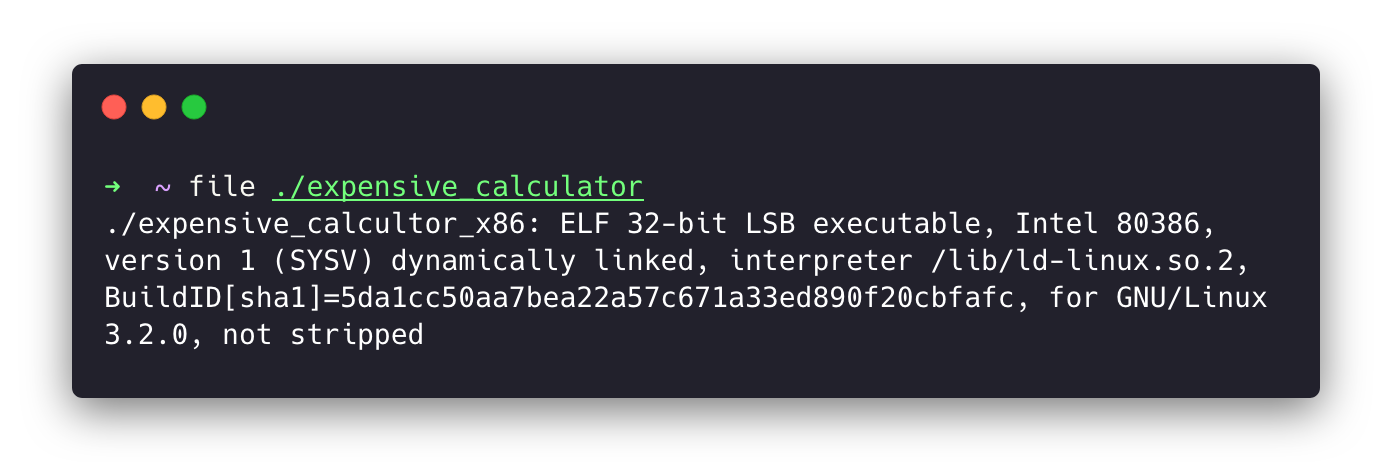
\includegraphics[width=0.8\textwidth]{figures/file_expensive}
  \caption{File properties}
  \label{f:file_expensive}
\end{figure}

The output of the file appears to be a 32 bit Linux executable with debug
symbols (not stripped). Debug Symbols will make the executable simpler to
understand and debug. Let's run the executable and see what it wants, and using
our intuition, we could see what inputs could cause the program to crash and how
to take advantage of this. After running the application, we get this. The
application wants a valid license key to proceed.
\begin{figure}[H]
  \centering
  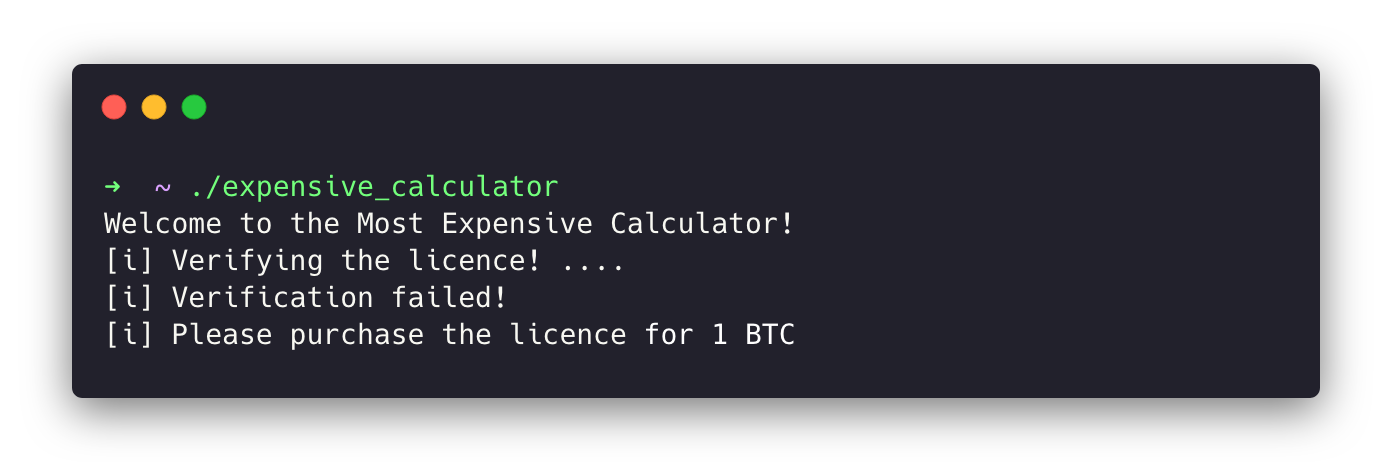
\includegraphics[width=0.8\textwidth]{figures/run_file}
  \caption{Execution of the file}
  \label{f:run_file}
\end{figure}
We need to know what it wants and give it to satisfy conditions required by the
application for a valid license key. Since it is an executable, let's
disassemble it and understand it in depth using static analysis. Opening the
file in IDA Pro, we start from the main and see what functions it calls from
there. Once IDA has disassembled and analysed the executable,we will look for
the main function in the left navigator and click on it.

\begin{figure}[H]
  \centering
  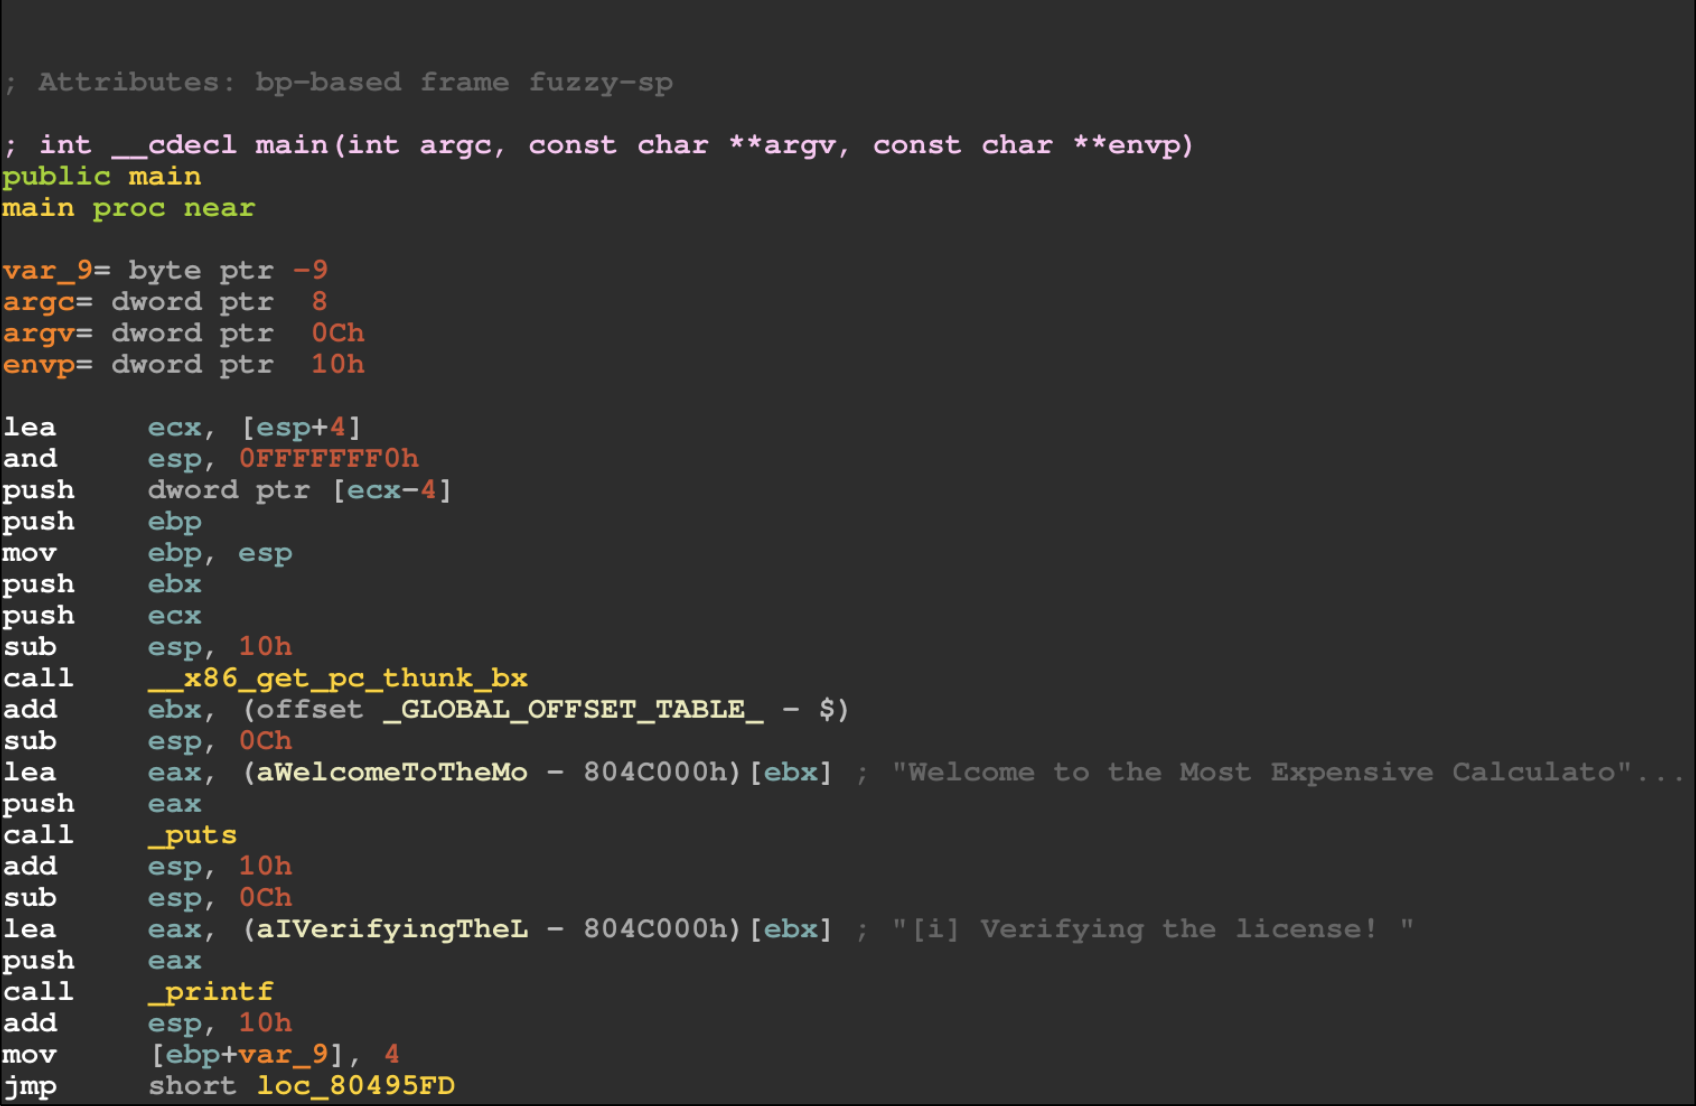
\includegraphics[width=0.8\textwidth]{figures/ida-main}
  \caption{IDA: main}
  \label{f:ida-main}
\end{figure}

To speed up reversing, the decompiler has been used. The code below is the
decompiled main function.
\begin{figure}[H]
  \centering
  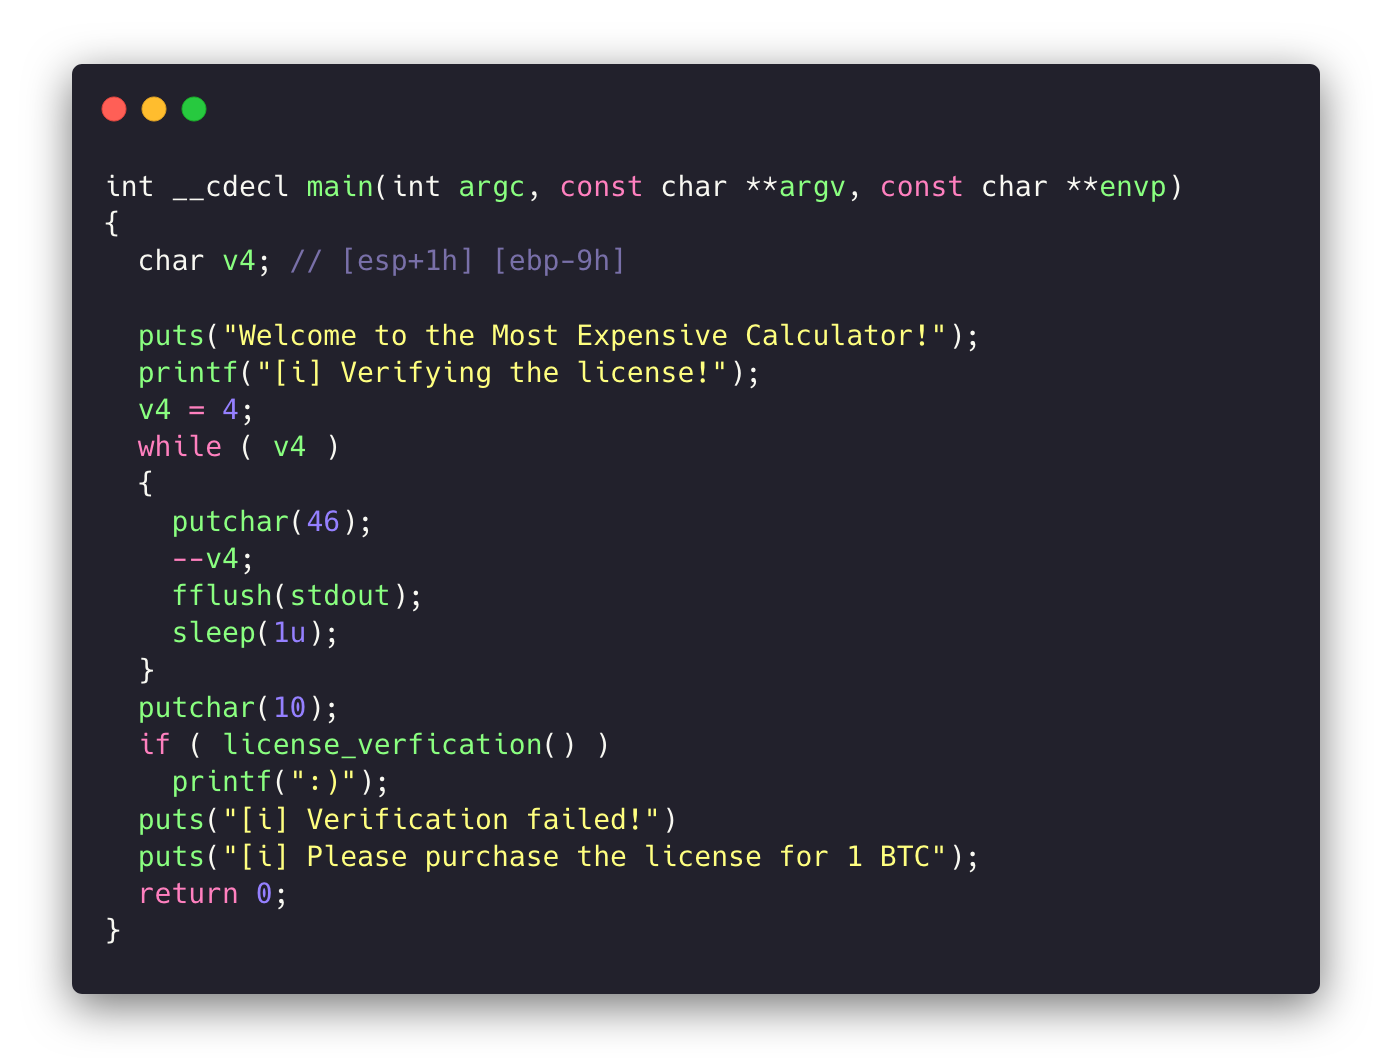
\includegraphics[width=0.8\textwidth]{figures/main-decompiled}
  \caption{Decompiled main}
  \label{f:main-decompiled}
\end{figure}

The most interesting part about the main is the license\_verification return
value. Let's investigate further.

\begin{figure}[H]
  \centering
  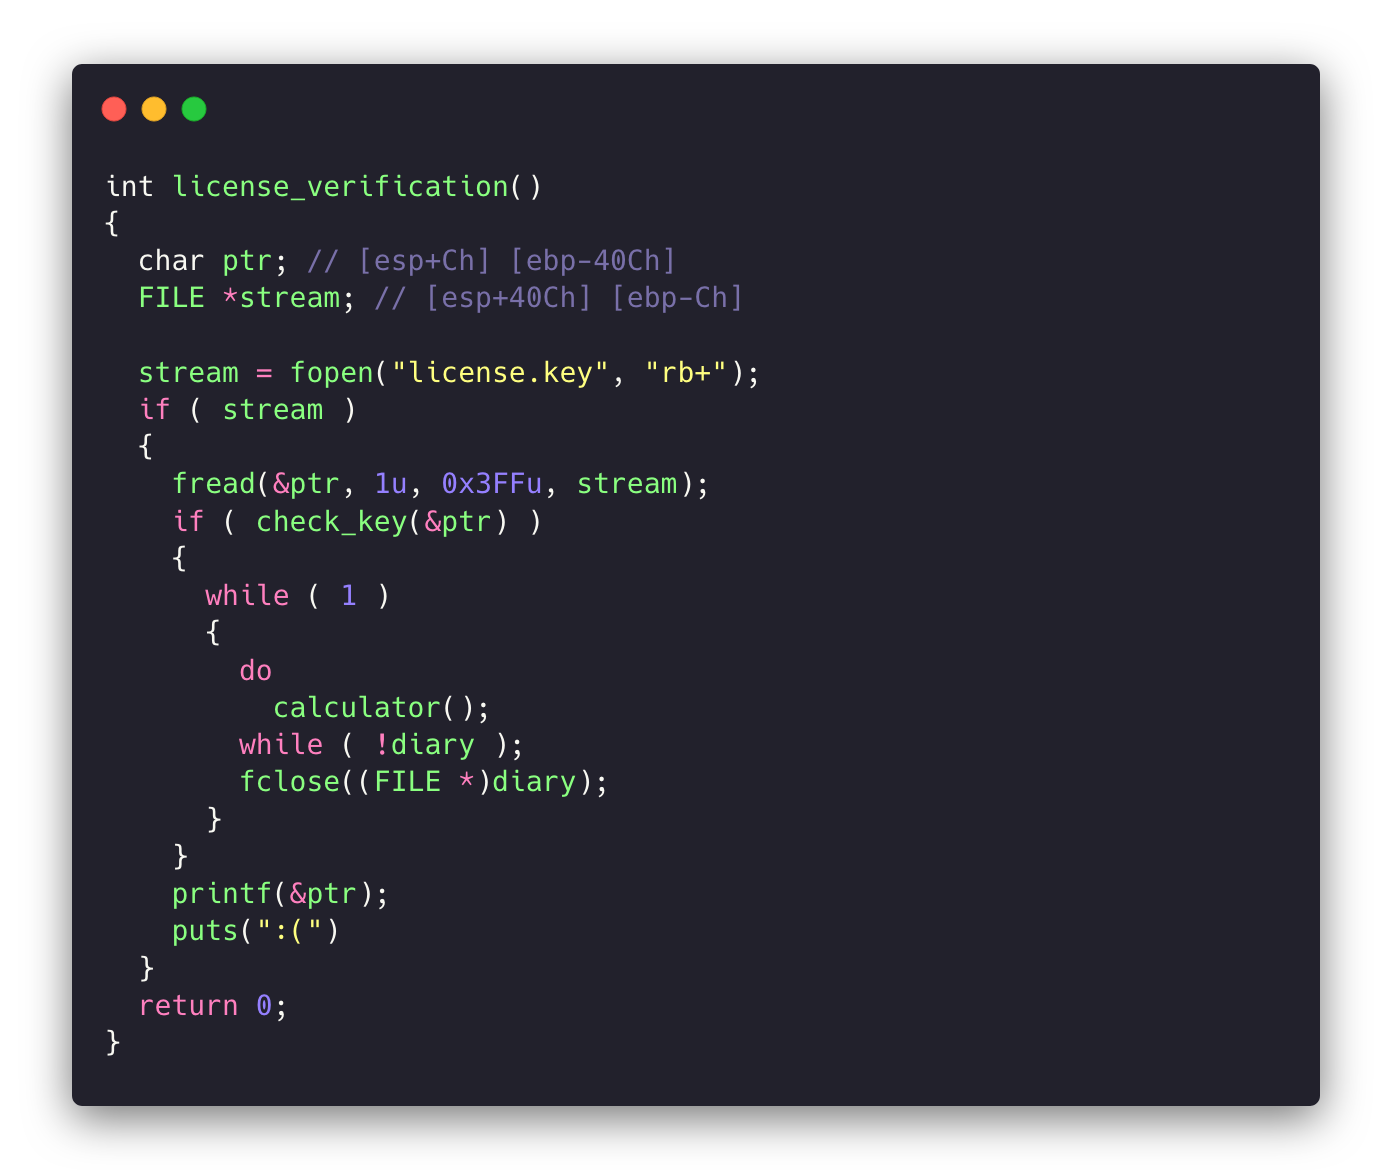
\includegraphics[width=0.8\textwidth]{figures/license-verification}
  \caption{License verification}
  \label{f:license-verification}
\end{figure}

The code tells us that a file ``license.key'` needs to be read and the contents
are stored in ``ptr''. After that, this array of chars is passed to
check\_key. If the return value of check\_key is non zero, then the calculator
runs until diary is closed. Let's take a look at check\_key.

\begin{figure}[H]
  \centering
  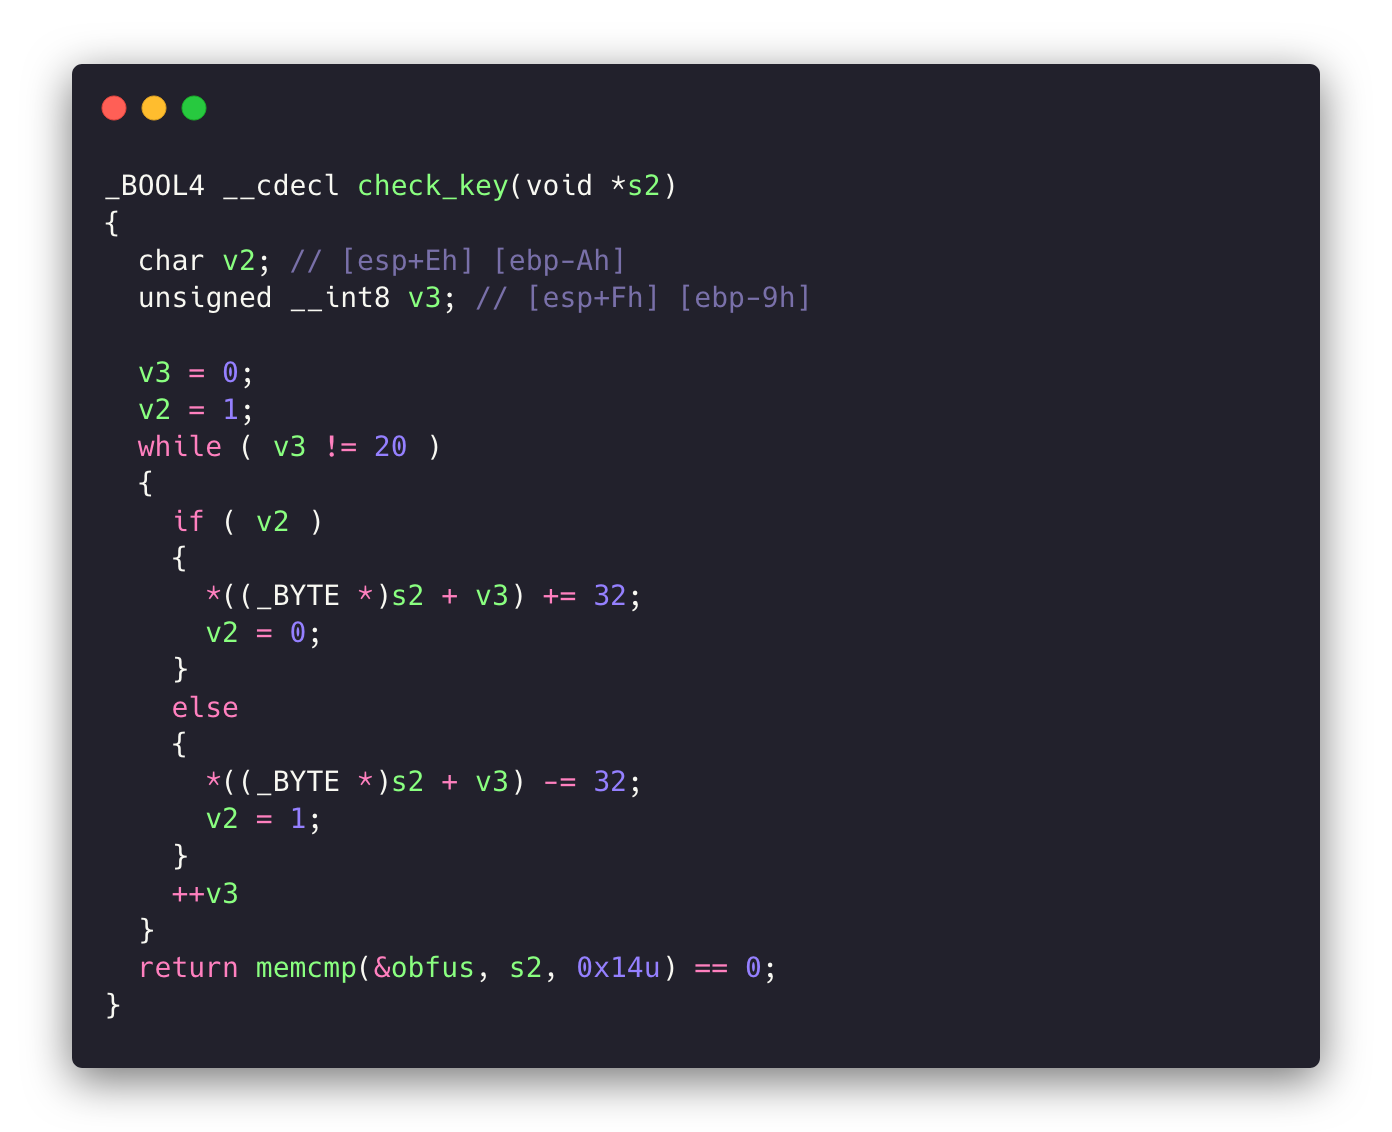
\includegraphics[width=0.7\textwidth]{figures/check-key}
  \caption{Check key}
  \label{f:check-key}
\end{figure}

Looking at this, the function wants the provided key characters added or
subtracted by 32 depending on their positions to match the obfus global variable.
For example, if the key is the password, what matches with obfus the first
character is int(`p') + 32 and the second character int(`a') - 32 should match
with the second obfus character so forth. This happens because, in the while
loop, v2 is checked if it is non zero. Then, the key's character at the current
position v3 is incremented by 32; otherwise, it is decremented. To crack this,
we add or subtract the 20 characters in obfus depending on its position and have
the key. For this we take the character values of obfus and store them in an
array. Clicking on the obfus on IDA, it will display its memory layout as below.

\begin{figure}[H]
  \centering
  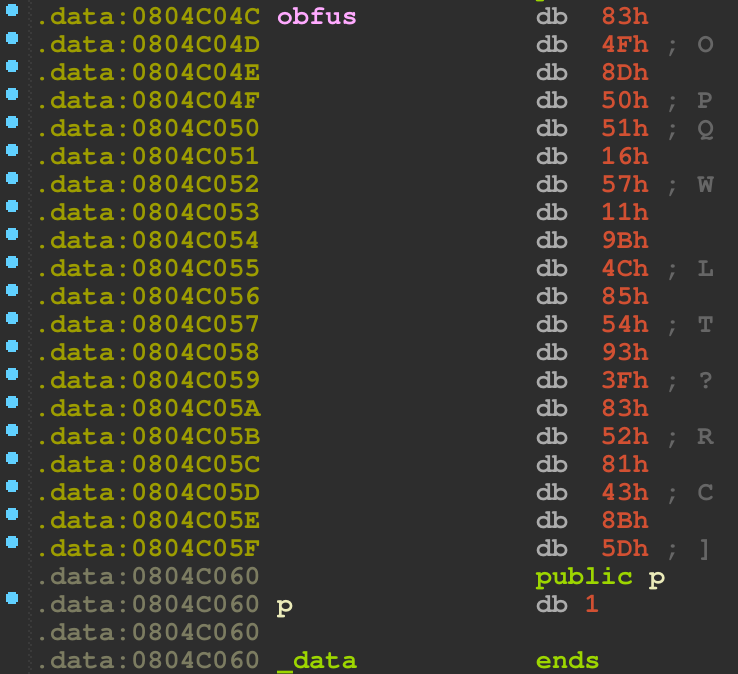
\includegraphics[width=0.4\textwidth]{figures/obfus}
  \caption{IDA: obfus}
  \label{f:obfus}
\end{figure}

Knowing this, we take the 20 bytes of the key and store them in a python list,
converting the logic previously described into code that manipulates it.

\begin{figure}[H]
  \centering
  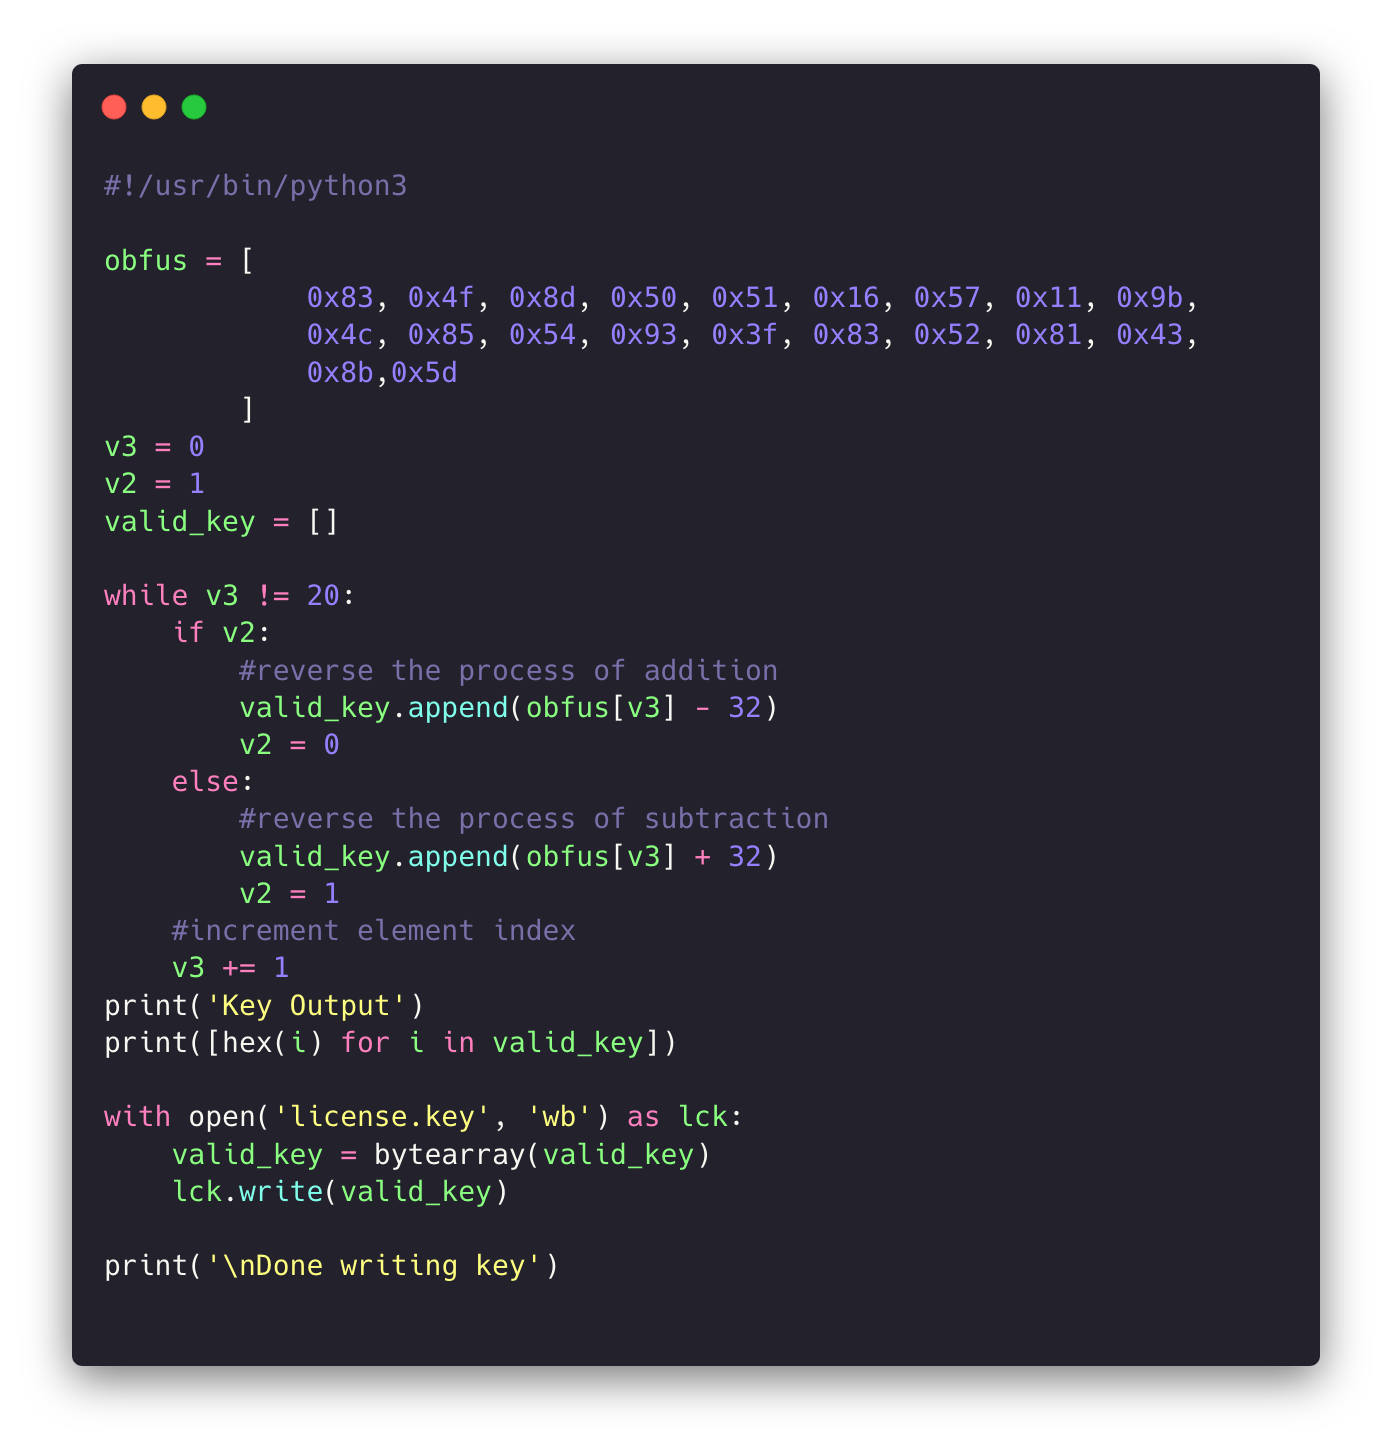
\includegraphics[width=0.8\textwidth]{figures/crack-license}
  \caption{Python script to crack the key}
  \label{f:crack-license}
\end{figure}

Running the script will generate the key in a license.key file. The output is
the following.

\begin{figure}[H]
  \centering
  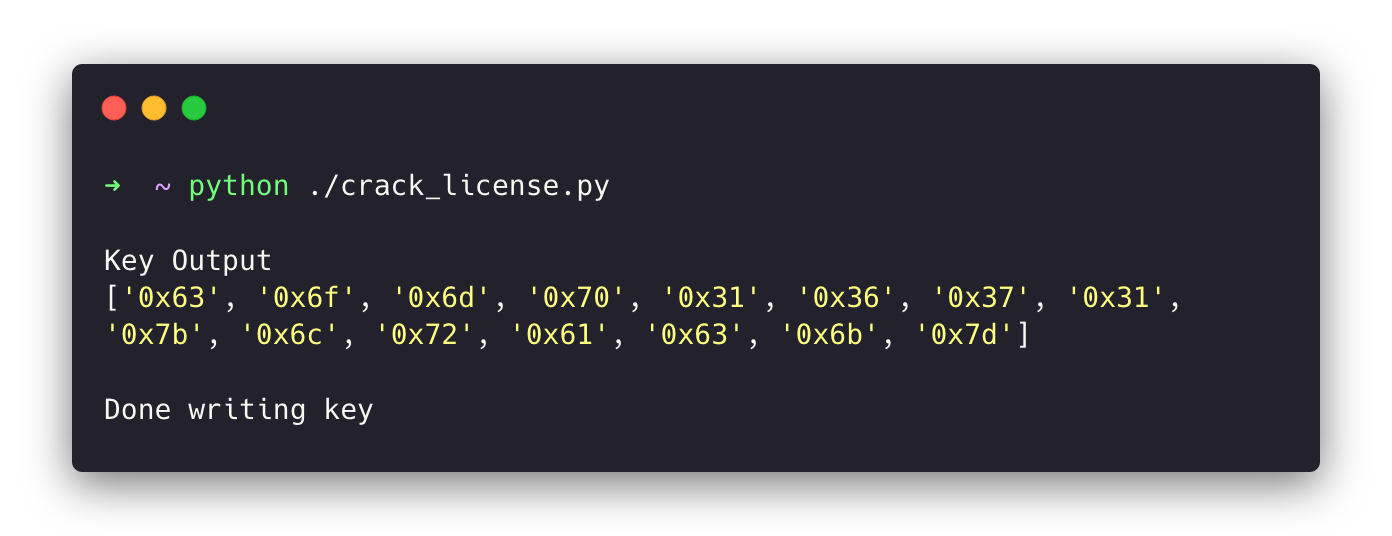
\includegraphics[width=0.8\textwidth]{figures/run-crack}
  \caption{Cracking the key}
  \label{f:run-crack}
\end{figure}

There is no error and the license.key file has been created. Let's have a look
at the content!

\begin{figure}[H]
  \centering
  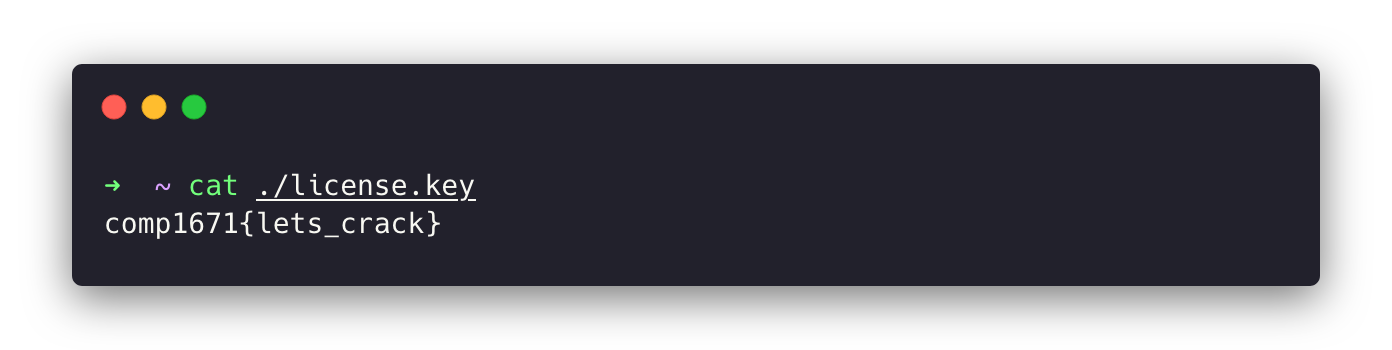
\includegraphics[width=0.8\textwidth]{figures/flag}
  \caption{Flag!}
  \label{f:flag}
\end{figure}

The key has been cracked and it is the flag!

\section{Conclusion}
\label{s:conclusion-lab-5}
RE is a very useful skill to have. The logic in an software can be cracked and
broken into pieces where informations that developers wanted to keep secret
could be found such as keys or secrets to APIs and databases. It requires a bit
of Assembly knowledge and understanding the logic behind everything could be a
bit overwhelming but with the right tools and motivation, it can be a very fun
exercise.
